% !TeX root = ../Book1.tex
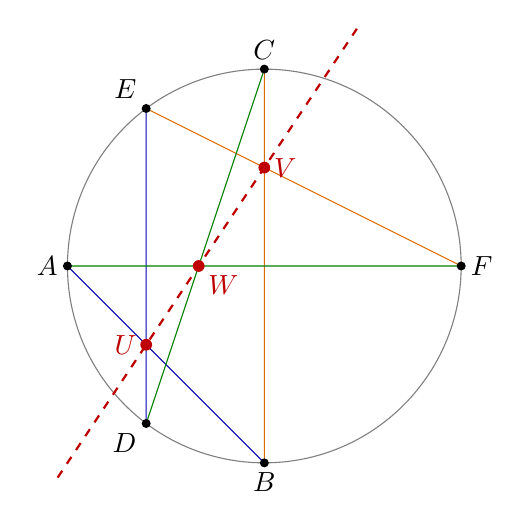
\begin{tikzpicture}[scale=2.5]
	\coordinate (A) at (-1,0);
	\coordinate (B) at (0,-1);
	\coordinate (C) at (0,1);
	\coordinate (D) at (-0.6,-0.8);
	\coordinate (E) at (-0.6,0.8);
	\coordinate (F) at (1,0);
	\draw[gray] (0,0) circle (1);
	\draw[blue!70!black] (A)--(B) (D)--(E);
	\draw[orange!85!black] (B)--(C) (E)--(F);
	\draw[green!50!black] (C)--(D) (F)--(A);
	\draw[red!75!black,thick,dashed] (-1.05,-1.075)--(0.47,1.205);
	\fill (A) circle (0.65pt) node[left]{\(A\)};
	\fill (B) circle (0.65pt) node[below]{\(B\)};
	\fill (C) circle (0.65pt) node[above]{\(C\)};
	\fill (D) circle (0.65pt) node[below left]{\(D\)};
	\fill (E) circle (0.65pt) node[above left]{\(E\)};
	\fill (F) circle (0.65pt) node[right]{\(F\)};
	\fill[red!75!black] (-0.6,-0.4) circle (0.85pt) node[left]{\(U\)};
	\fill[red!75!black] (0,0.5) circle (0.85pt) node[right]{\(V\)};
	\fill[red!75!black] (-0.333333,0) circle (0.85pt) node[below right]{\(W\)};
\end{tikzpicture}
